%% 
%% Copyright 2007-2020 Elsevier Ltd
%% 
%% This file is part of the 'Elsarticle Bundle'.
%% ---------------------------------------------
%% 
%% It may be distributed under the conditions of the LaTeX Project Public
%% License, either version 1.2 of this license or (at your option) any
%% later version.  The latest version of this license is in
%%    http://www.latex-project.org/lppl.txt
%% and version 1.2 or later is part of all distributions of LaTeX
%% version 1999/12/01 or later.
%% 
%% The list of all files belonging to the 'Elsarticle Bundle' is
%% given in the file `manifest.txt'.
%% 

%% Template article for Elsevier's document class `elsarticle'
%% with numbered style bibliographic references
%% SP 2008/03/01
%%
%% 
%%
%% $Id: elsarticle-template-num.tex 190 2020-11-23 11:12:32Z rishi $
%%
%%
\documentclass[preprint,12pt]{elsarticle}

%% Use the option review to obtain double line spacing
%% \documentclass[authoryear,preprint,review,12pt]{elsarticle}

%% Use the options 1p,twocolumn; 3p; 3p,twocolumn; 5p; or 5p,twocolumn
%% for a journal layout:
%% \documentclass[final,1p,times]{elsarticle}
%% \documentclass[final,1p,times,twocolumn]{elsarticle}
%% \documentclass[final,3p,times]{elsarticle}
%% \documentclass[final,3p,times,twocolumn]{elsarticle}
%% \documentclass[final,5p,times]{elsarticle}
%% \documentclass[final,5p,times,twocolumn]{elsarticle}

%% For including figures, graphicx.sty has been loaded in
%% elsarticle.cls. If you prefer to use the old commands
%% please give \usepackage{epsfig}

%% The amssymb package provides various useful mathematical symbols
\usepackage{amssymb}
%% The amsthm package provides extended theorem environments
%% \usepackage{amsthm}
\usepackage{amsfonts,amsmath,amscd}
\usepackage{float}
\usepackage{graphicx}
\usepackage{subfig}
\usepackage{nccmath}
% \usepackage[authoryear]{natbib}
% For degree symbol
\usepackage{siunitx}
\usepackage{booktabs}
\usepackage{url}

%% The lineno packages adds line numbers. Start line numbering with
%% \begin{linenumbers}, end it with \end{linenumbers}. Or switch it on
%% for the whole article with \linenumbers.
%% \usepackage{lineno}

% \journal{Pattern Recognition}

\begin{document}

\begin{frontmatter}

%% Title, authors and addresses

%% use the tnoteref command within \title for footnotes;
%% use the tnotetext command for theassociated footnote;
%% use the fnref command within \author or \address for footnotes;
%% use the fntext command for theassociated footnote;
%% use the corref command within \author for corresponding author footnotes;
%% use the cortext command for theassociated footnote;
%% use the ead command for the email address,
%% and the form \ead[url] for the home page:
%% \title{Title\tnoteref{label1}}
%% \tnotetext[label1]{}
%% \author{Name\corref{cor1}\fnref{label2}}
%% \ead{email address}
%% \ead[url]{home page}
%% \fntext[label2]{}
%% \cortext[cor1]{}
%% \affiliation{organization={},
%%             addressline={},
%%             city={},
%%             postcode={},
%%             state={},
%%             country={}}
%% \fntext[label3]{}

\title{An Intuitive Tutorial to Gaussian Processes Regression}

%% use optional labels to link authors explicitly to addresses:
%% \author[label1,label2]{}
%% \affiliation[label1]{organization={},
%%             addressline={},
%%             city={},
%%             postcode={},
%%             state={},
%%             country={}}
%%
%% \affiliation[label2]{organization={},
%%             addressline={},
%%             city={},
%%             postcode={},
%%             state={},
%%             country={}}

\author[label1]{Jie Wang \corref{cor1}}
\ead{jwangjie@outlook.com}
\cortext[cor1]{Corresponding author}

\affiliation[label1]{organization={Ingenuity Labs Research Institute, Queen's University},%Department and Organization
            addressline={69 Union St~W}, 
            city={Kingston},
            postcode={K7L~3N6}, 
            state={ON},
            country={Canada}}

\begin{abstract}
This tutorial aims to provide an intuitive understanding of the Gaussian processes regression. Gaussian processes regression (GPR) models have been widely used in machine learning applications because of their representation flexibility and inherent uncertainty measures over predictions. The basic concepts that a Gaussian process is built on, including multivariate normal distribution, kernels, non-parametric models, and joint and conditional probability were explained first. Next, the GPR was described concisely together with an implementation of a standard GPR algorithm. Beyond the standard GPR, packages to implement state-of-the-art Gaussian processes algorithms were reviewed. This tutorial was written in an accessible way to make sure readers without a machine learning background can obtain a good understanding of the GPR basics. 
\end{abstract}

% %%Graphical abstract
% \begin{graphicalabstract}
% %\includegraphics{grabs}
% 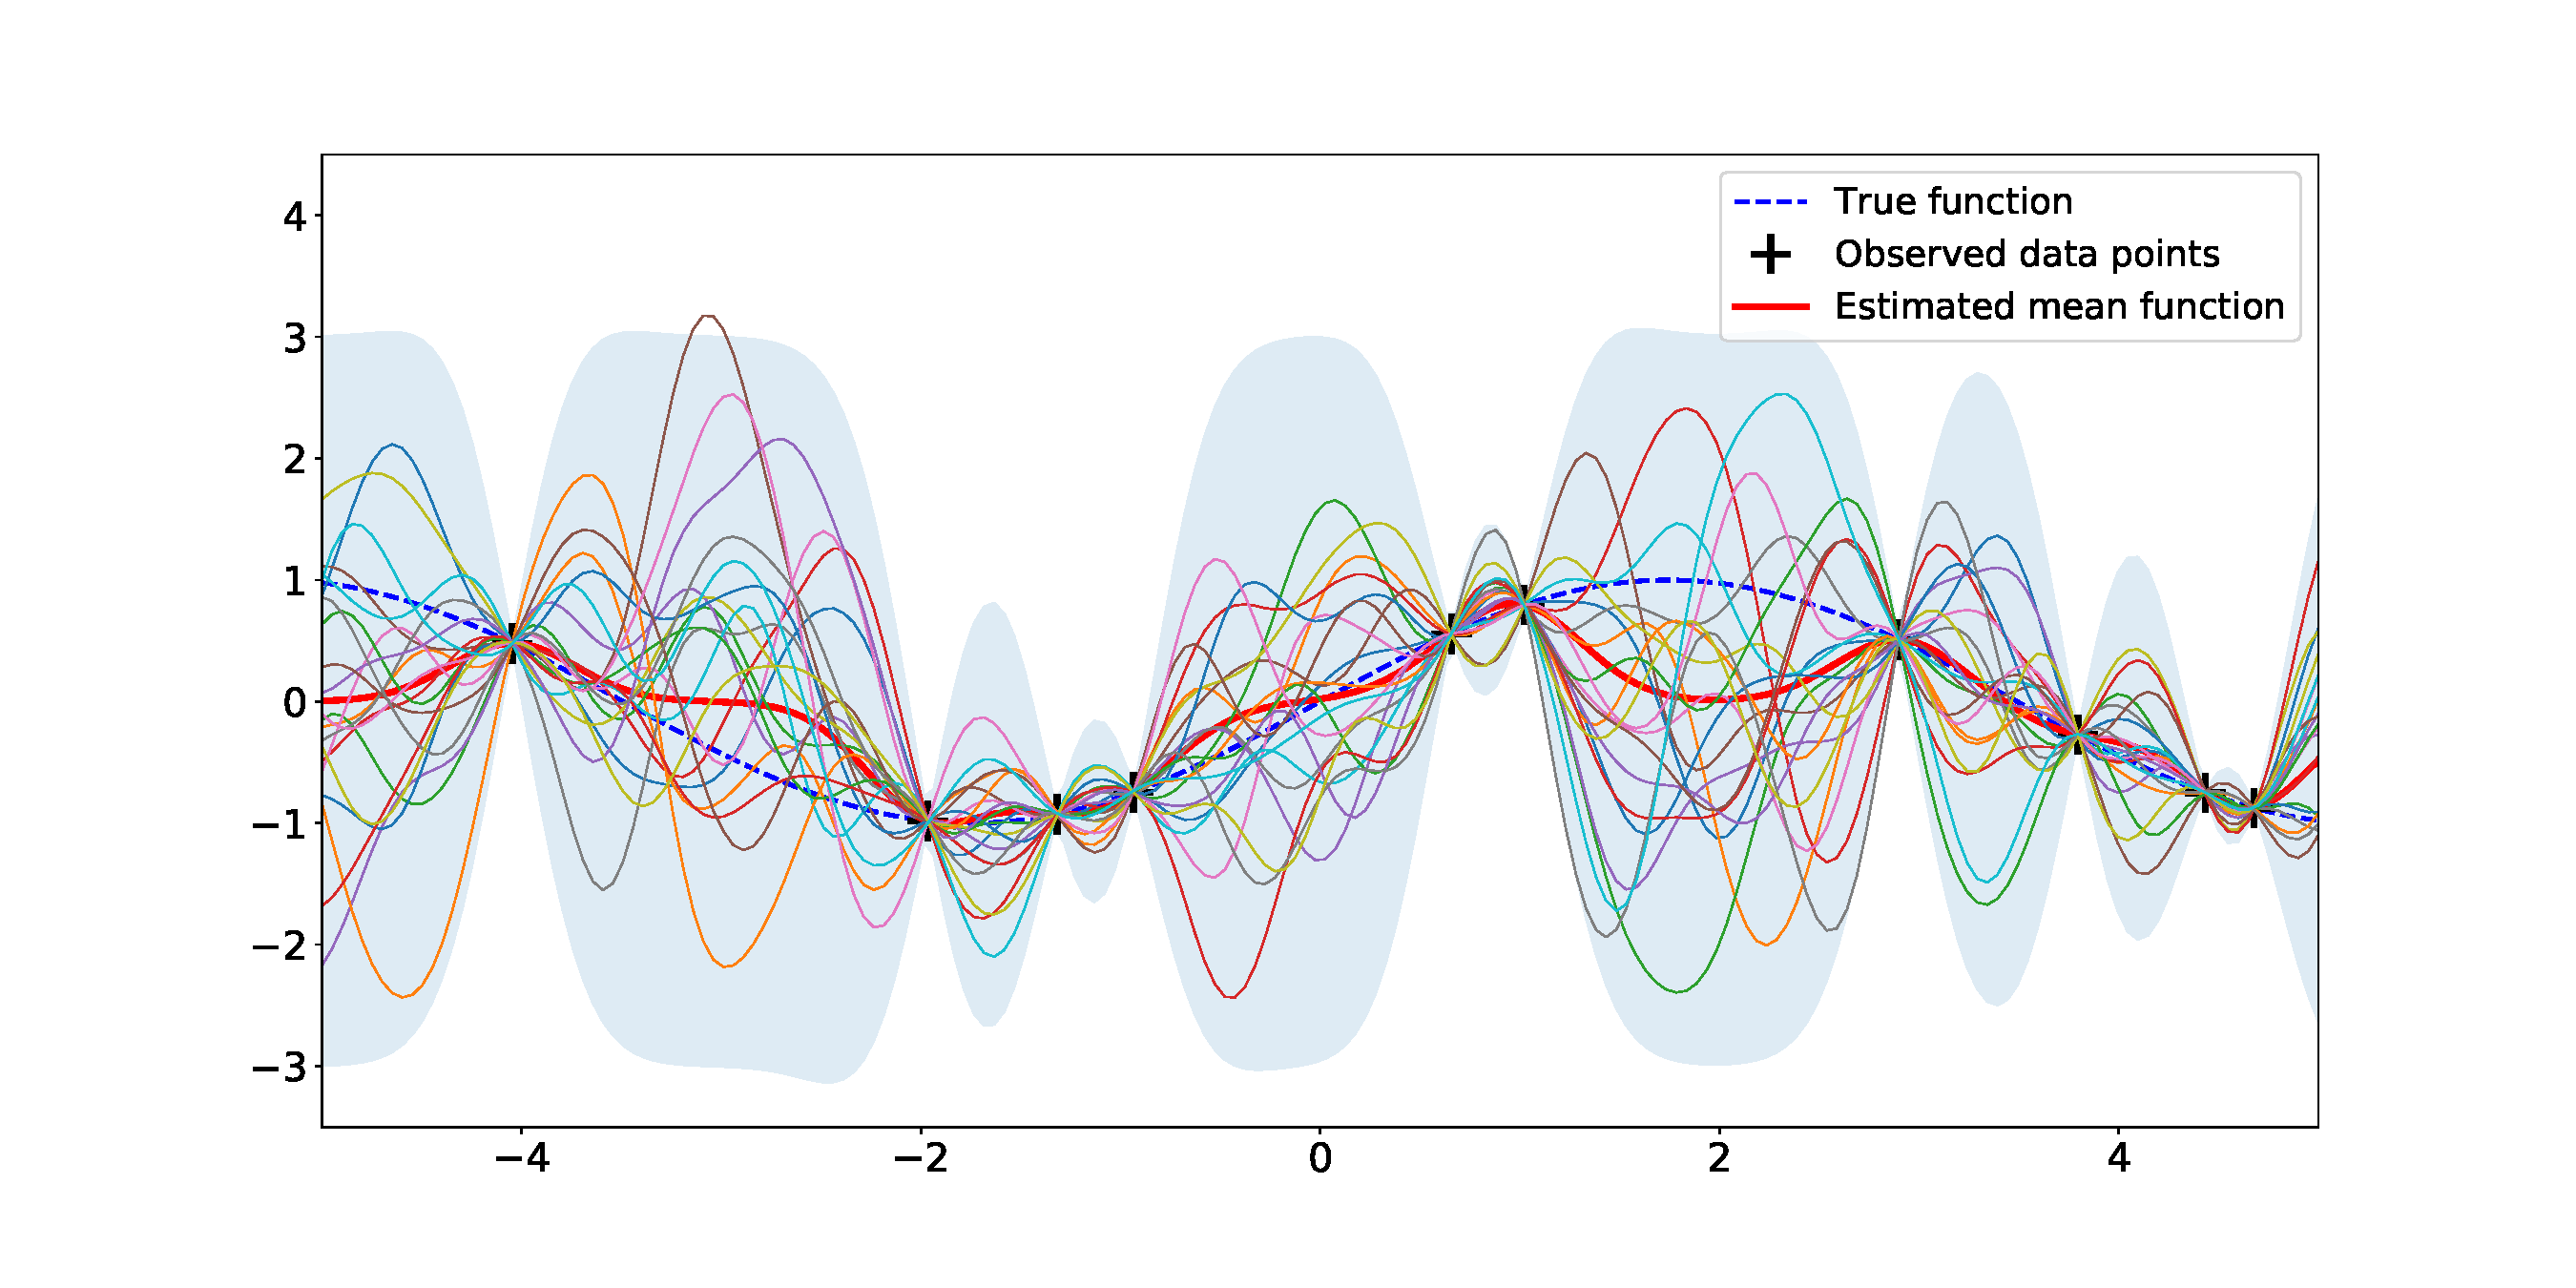
\includegraphics[trim=4.5cm 2.0cm 4.4cm 0.6cm, width=\textwidth]{figs/illustrative_posterior_func.pdf}
% \end{graphicalabstract}

% \begin{highlights}
% \item Explained the basic concepts that a Gaussian process is built on in an accessible way.
% \item Described and implemented the standard Gaussian processes regression. 
% \item Provided accompany codes of the plots showed in this paper. 
% \end{highlights}

\begin{keyword}
%% keywords here, in the form: keyword \sep keyword
Gaussian Processes Regression \sep Multivariate Normal Distribution \sep Kernels \sep  Hyperparameters \sep Gaussian Processes Packages 
\end{keyword}

\end{frontmatter}

%% \linenumbers

%% main text
\section{Introduction}
The Gaussian processes model is a probabilistic supervised machine learning framework that has been widely used for regression and classification tasks. A Gaussian processes regression (GPR) model can make predictions incorporating prior knowledge (kernels) and provide uncertainty measures over predictions \cite{Rasmussen2006}. Gaussian processes model is a supervised learning method developed by computer science and statistics communities. Researchers with engineering backgrounds often find it difficult to gain a clear understanding of it. To understand GPR, even only the basics need to have knowledge of multivariate normal distribution, kernels, non-parametric model, and joint and conditional probability. 

In this tutorial, we present a concise and accessible explanation of GPR. We first review the mathematical concepts that GPR models are built on to make sure readers have enough basic knowledge. In order to provide an intuitive understanding of GPR, plots are actively used. The codes developed to generate plots are provided at \url{https://github.com/jwangjie/Gaussian-Processes-Regression-Tutorial}. 

\section{Mathematical Basics}
This section reviews the basic concepts needed to understand GPR. We start with the Gaussian (normal) distribution, then explain theories of multivariate normal distribution (MVN), kernels, non-parametric model, and joint and conditional probability. In regression, given some observed data points, we want to fit a function to represent these data points, then use the function to make predictions at new data points. For a given set of observed data points shown in Fig. \ref{FIG:1}(a), there are infinite numbers of possible functions that fit these data points. In Fig. \ref{FIG:1}(b), we show five sample functions that fit the data points. In GPR, the Gaussian processes conduct regression by defining a distribution over these infinite number of functions \cite{ghahramani2011tutorial}.

\begin{figure}[h!]
    \centering
    \subfloat[Data point observations]{{\includegraphics[trim=2.0cm 0.8cm 3.2cm 1.8cm, width=6.3cm]{figs/regression_points.pdf} }}
    \qquad
    \subfloat[Five possible functions by GPR]{{\includegraphics[trim=2.0cm 0.8cm 3.2cm 1.8cm, width=6.3cm]{figs/regression.pdf} }}
    \caption{A regression example: (a) The observed data points, (b) Five sample functions that fit the observed data points.}%
    \label{FIG:1}
\end{figure}

\subsection{Gaussian Distribution}

A random variable $X$ is Gaussian or normally distributed with mean $\mu$ and variance $\sigma^2$ if its probability density function (PDF) is \cite{Murphy2012}

\begin{ceqn}
    \begin{align}
       P_X(x) = \frac{1}{\sqrt{2 \pi} \sigma} exp{\left(-\frac{{\left(x - \mu \right)}^{2}}{2 \sigma^{2}}\right)} \ . \nonumber
    \end{align}
\end{ceqn}
Here, $X$ represent random variables and $x$ is the real argument. The normal distribution of $X$ is usually represented by $ P_X(x) ~ \sim\mathcal{N}(\mu, \sigma^2)$. The PDF of a uni-variate normal (or Gaussian) distribution was plotted in Fig. \ref{FIG:2}. We randomly generated 1000 points from a uni-variate normal distribution and plotted them on the $x$ axis.

\begin{figure}[h!]
	\centering
		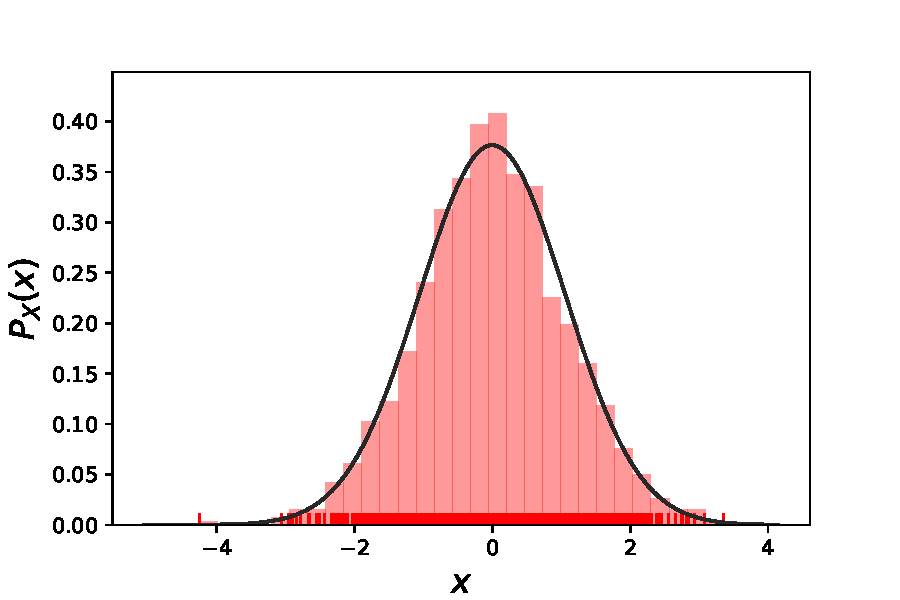
\includegraphics[trim=0.4cm 0.1cm 1.4cm 0.6cm, width=0.6\textwidth]{figs/1d_random.pdf}
    	\caption{One thousand normal distributed data points were plotted as red vertical bars on the $x$ axis. The PDF of these data points was plotted as a two-dimensional bell curve.}
    	\label{FIG:2}
\end{figure}

These random generated data points can be expressed as a vector $x_1=[x_1^1, x_1^2, \ldots, x_1^n]$. By plotting the vector $x_1$ on a new $Y$ axis at $Y = 0$, we projected points $[x_1^1, x_1^2, \ldots, x_1^n]$ into another space shown in Fig. \ref{FIG:3}. We did nothing but vertically plot points of the vector $x_1$ in a new $Y, x$ coordinates space. We can plot another independent Gaussian vector $x_2=[x_2^1, x_2^2, \ldots, x_2^n]$ in the same coordinates at $Y = 1$ shown in Fig. \ref{FIG:3}. Keep in mind that either $x_1$ or $x_2$ is a uni-variate normal distribution shown in Fig. \ref{FIG:2}. 

\begin{figure}[h!]
	\centering
		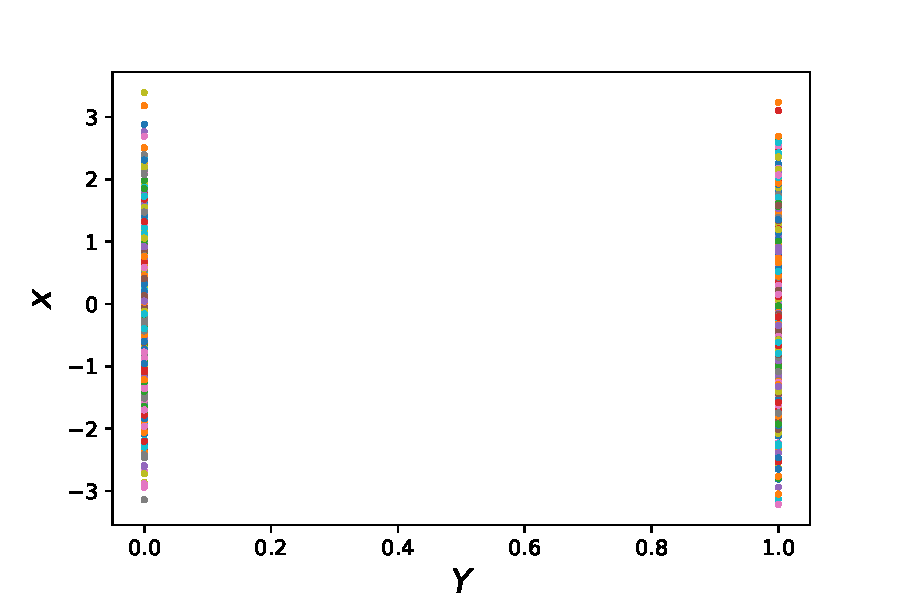
\includegraphics[width=0.7\textwidth]{figs/2gaussian.pdf}
	\caption{Two independent uni-variate Gaussian vector points were plotted vertically in the $Y, x$ coordinates space.}
	\label{FIG:3}
\end{figure}

Next, we randomly selected 10 points in vector $x_1$ and $x_2$ respectively and connected these 10 points in order by lines as shown in Fig. \ref{FIG:4}(a). These connected lines look like linear functions spanning within the $[0, 1]$ domain. We can use these functions to make predictions for regression tasks if the new data points are on (or close enough to) these linear lines. However, in most cases, the assumption that new data points are always on the connected linear functions is not held. If we plot more random generated uni-variate Gaussian vectors, for example, 20 vectors $x_1, x_2, \ldots, x_{20}$ in $[0, 1]$, and connect 10 random selected sample points of each vector as lines, we get 10 lines that look more like functions within $[0, 1]$ shown in Fig. \ref{FIG:4}(b). We still cannot use these lines to make predictions for regression tasks because they are too noisy. These functions must be smoother, meaning input points that are close to each other should have similar output values. The``functions'' generated by connecting independent Gaussian vector points are not smooth enough for regression tasks, we need these independent Gaussian correlated to each other as a joint Gaussian distribution. The joint Gaussian distribution is described by the multivariate normal distribution theory.  

\begin{figure}[h!]
    \centering
    \subfloat[Two Gaussian vectors]{{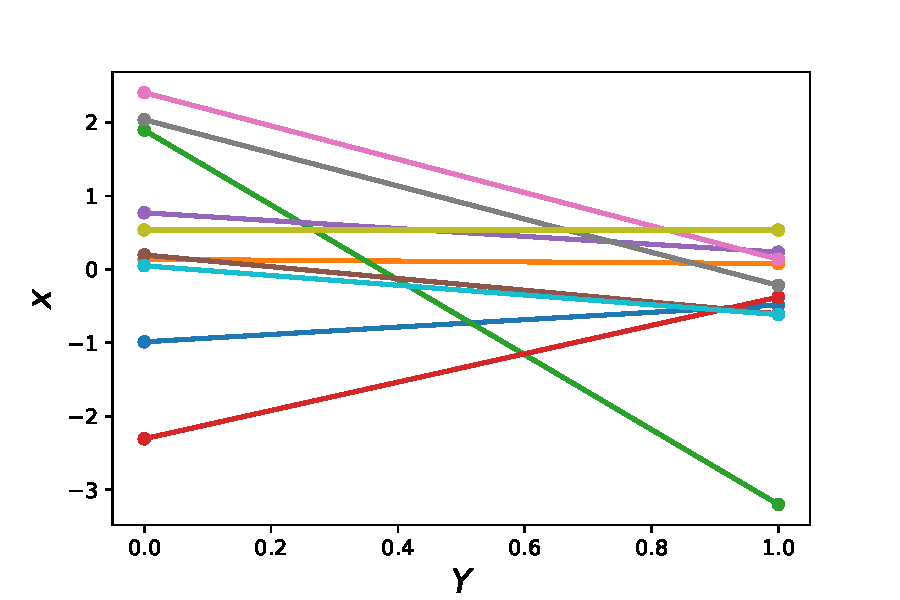
\includegraphics[trim=0.3cm 0.1cm 1.6cm 1.1cm, width=6.32cm]{figs/random_x1_x2.pdf} }}
    \qquad
    \subfloat[Twenty Gaussian vectors]{{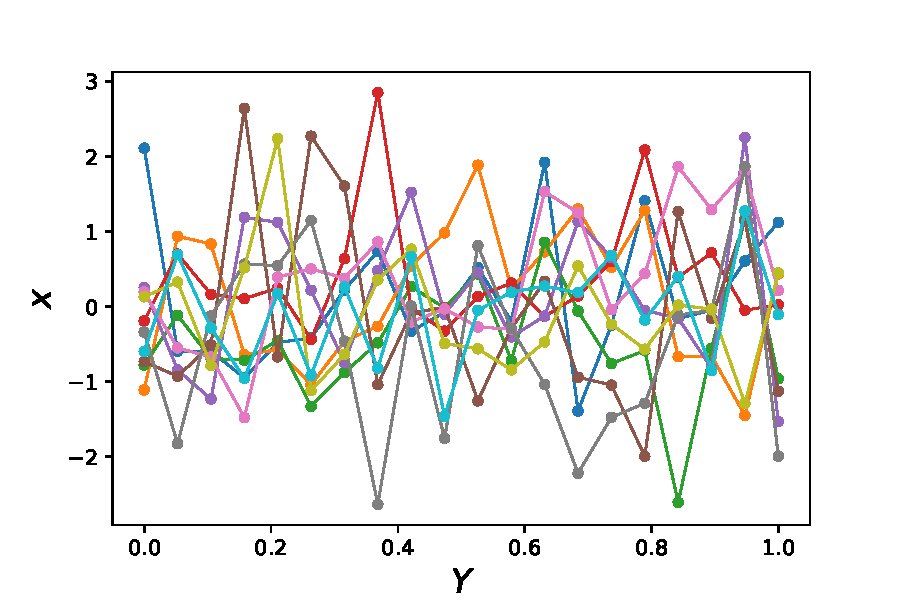
\includegraphics[trim=0.6cm 0.1cm 1.6cm 1.1cm, width=6.22cm]{figs/random_x1_x20.pdf} }}
    \caption{Connecting points of independent Gaussian vectors by lines: (a) Ten random selected points in two vector $x_1$ and $x_2$ , (b) Ten random selected points in twenty vectors $x_1, x_2, \ldots, x_{20}$ .}
    \label{FIG:4}
\end{figure}

\subsection{Multivariate Normal Distribution}

It's common that a system is described by more than one feature variables $(x_1, x_2, \ldots, x_D)$ that are correlated to each other. If we want to model these variables all together as one Gaussian model, we need to use a multivariate Gaussian/normal (MVN) \cite{Murphy2012} distribution model. The PDF of an MVN with D dimension is defined as \cite{Murphy2012}
\begin{ceqn}
    \begin{align}
       \mathcal{N}(x | \mu,\Sigma) = \dfrac{1}{(2\pi)^{D/2}|\Sigma|^{1/2}}\exp\left[-\dfrac{1}{2}(x-\mu)^\mathsf{T} \Sigma^{-1}(x-\mu)\right] \ , \nonumber
    \end{align}
\end{ceqn}
where $D$ is the number of the dimension, $x$ represents the variable, $\mu=\mathbb{E}[x] \in \mathbb{R}^D$ is the mean vector, and $\Sigma=\text{cov}[x]$ is the $D \times D$ covariance matrix. The $\Sigma$ is a symmetric matrix that stores the pairwise covariance of all jointly modeled random variables with $\Sigma_{ij}=\text{cov}(y_i,y_j)$ as its $(i,j)$ element. 
\\
\\
\begin{figure}[h!]
    \centering
    \subfloat[3-d bell curve]{{\includegraphics[trim=1.6cm 1.0cm 2.6cm 2.0cm, width=0.56\textwidth]{figs/3d_gaussian_example.pdf} }}
    \qquad
    \subfloat[2-d ellipse contours]{{\includegraphics[trim=0.3cm 0.0cm 0.8cm 0.6cm, width=0.35\textwidth]{figs/2d_gaussian_example.pdf} }}
    \caption{The PDF of a BVN visualization: (a) a 3-d bell curve with height represents the probability density, (b) ellipse contour projections showing the co-relationship between $x_1$and $x_2$ points.}%
    \label{FIG:5}
\end{figure}

We use a bi-variate normal (BVN) distribution as a simplified example to understand the MVN theory. A BVN distribution can be visualized as a three-dimensional (3-d) bell curve with heights represent the probability density shown in Fig. \ref{FIG:5}a. The projections of the 3-d bell curve on the $x_1, x_2$ plane are ellipse contours plotted in Fig. \ref{FIG:5}a and \ref{FIG:5}b. The shape of ellipses shows the correlations between $x_1$ and $x_2$ points, i.e. how much one variable of $x_1$ is related to another variable of $x_2$. The $P(x_1, x_2)$ is the joint probability of $x_1$ and $x_2$. For a BVN, the mean vector $\mu$ is a two-dimensional vector $\begin{bmatrix} \mu_1 \\ \mu_2 \end{bmatrix}$, where $\mu_1$ and $\mu_2$ are the independent mean of $x_1$ and $x_2$ respectively. The covariance matrix is $\begin{bmatrix} \sigma_{11} & \sigma_{12} \\ \sigma_{21} & \sigma_{22} \end{bmatrix}$, where the diagonal terms $\sigma_{11}$ and $\sigma_{22}$ are the independent variance of $x_1$ and $x_2$ respectively. The off-diagonal terms $\sigma_{12}$ and $\sigma_{21}$ represent correlations between $x_1$ and $x_2$. The BVN is expressed as 
\begin{ceqn}
    \begin{align}
       \begin{bmatrix} x_1 \\ x_2 \end{bmatrix} \sim \mathcal{N}\left(\begin{bmatrix} \mu_1 \\ \mu_2 \end{bmatrix}, \begin{bmatrix} \sigma_{11} & \sigma_{12}  \\ \sigma_{21} & \sigma_{22} \end{bmatrix}\right) \sim \mathcal{N}(\mu, \Sigma) \ . \nonumber
    \end{align}
\end{ceqn}

It is intuitively understandable that we need conditional probability rather than the joint probability for regression tasks. If we cut a slice on the 3-d bell curve shown in Fig. \ref{FIG:5}, we get the conditional probability distribution $P(x_1 \vert \, x_2)$ shown in Fig. \ref{FIG:6}. The conditional distribution is also Gaussian \cite{Rasmussen2006}.

\begin{figure}[h!]
	\centering
	\includegraphics[trim=0.4cm 0.4cm 0.6cm 0.8cm, width=0.68\textwidth]{figs/2d_gaussian_conditional.pdf}
	\caption{The conditional probability distribution $P(x_1 \vert \, x_2)$ by cutting a slice on the PDF 3-d bell curve of a BVN.}
	\label{FIG:6}
\end{figure}

\subsection{Kernels}

After reviewing the MVN concept, we want to smooth the functions in Fig. \ref{FIG:4}(b). This can be done by defining covariance functions, which reflect our ability to express prior knowledge of the form of the function we are modeling. In regression, outputs of the function should be similar when two inputs are close to each other. One possible equation format is the dot product $A \cdot B = \lVert A \rVert \lVert B \rVert \text{cos}\theta$, where $\theta$ is the angle between two input vectors. When two input vectors are similar, their dot product output value is high. 

If a function is defined solely in terms of inner products in the input space, then the function $k(x,\ x^\prime)$ is a kernel function \cite{Rasmussen2006}. The most widely used kernel or covariance function is the squared exponential (SE) kernel function. The SE kernel is de-facto default kernel for Gaussian processes \cite{duvenaud2014automatic}. This is because it can be integrated against most functions that you need to due to its universal property. And every function in its prior has infinitely many derivatives. It's also known as the radial basis function (RBF) kernel or Gaussian kernel function that is defined as \footnote{This is a simplified RBF without hyperparameters for simplicity. A general RBF will be further explained in section \ref{Hyperparameters}.} 
\begin{ceqn}
    \begin{align}
       \text{cov}(x_i, x_j)=\exp\left(-~\frac{(x_i-x_j)^2}{2}\right) \ . \nonumber
    \end{align}
\end{ceqn}

In Fig. \ref{FIG:4}(b), we plotted 20 independent Gaussian vectors by connecting 10 randomly selected sample points of each vector in order by lines. Instead of plotting 20 independent Gaussian, we generated 10 twenty-variate normal (20-VN) distributions with an identity covariance function shown in \ref{FIG:7}(a). It's the same as \ref{FIG:4}(b) due to there being no correlations between points by using identity as its kernel function. When an RBF was used as the covariance function, we got smooth lines shown in \ref{FIG:7}(b).

\begin{figure}[h!]
    \centering
    \subfloat[Ten samples of the 20-VN prior with an identity kernel]{{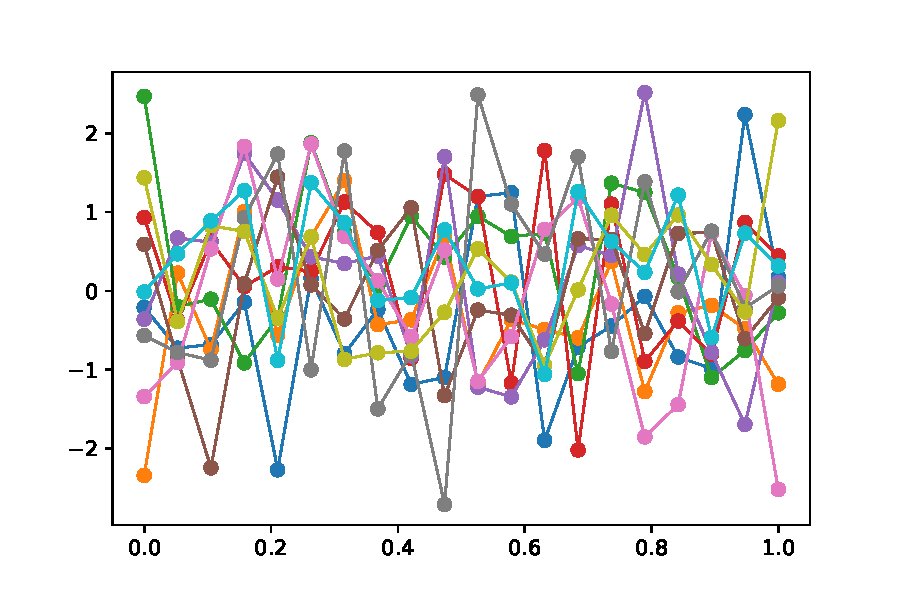
\includegraphics[trim=1.2cm 0.4cm 1.6cm 1.1cm, width=0.45\textwidth]{figs/20d_gaussian_prior.pdf} }}
    \qquad
    \subfloat[Ten samples of the 20-VN prior with a RBF kernel]{{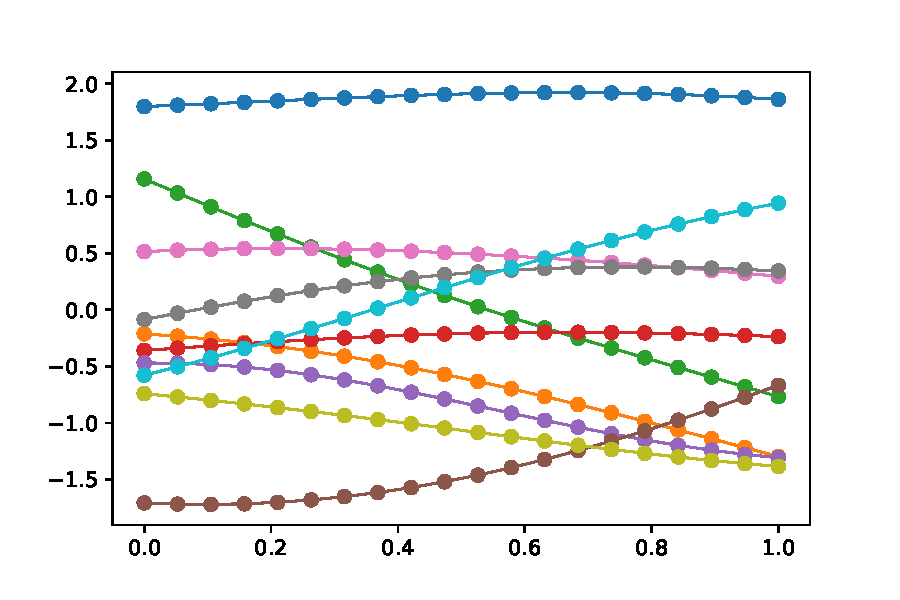
\includegraphics[trim=0.9cm 0.4cm 1.6cm 1.1cm, width=0.46\textwidth]{figs/20d_gaussian_kernel_prior.pdf} }}
    \caption{Samples of twenty-variate normal (20-VN) distribution kernelized prior functions: (a) Ten 20-VN with an identity function covariance, (b) Ten 20-VN with a RBF covariance.}
    \label{FIG:7}
\end{figure}

By adding covariance functions, we obtain smoother lines, and they start to look like functions. It is natural to consider continuing to increase the dimension of MVN. Here, dimension refers to the number of multi-variables of MVN. When the dimension of MVN gets larger, the region of interest will be filled up with more points. When the dimension becomes infinity, there will be a point to represent any possible input point. By using MVN with infinity dimensions, we fit functions with infinity parameters to do regression tasks. We can make predictions anywhere in the region of interest. In Fig. \ref{FIG:8}, We plotted 200 samples of a two hundred-variate normal (200-VN) distribution to get a feeling of functions with infinity parameters. We call these functions kernelized prior functions because there are no observed data points yet. All functions are randomly generated by the MVN model incorporating kernel functions as prior knowledge before having any observed data points. 

\begin{figure}[h!]
	\centering
		\includegraphics[width=\textwidth]{figs/200d_gaussian_kernel_prior.png}
	\caption{Two hundred kernelized prior functions of a two hundred-variate normal distribution.}
	\label{FIG:8}
\end{figure}

\subsection{Non-parametric Model}

This section explains the concept of parametric and nonparametric models \cite{Murphy2012}. Parametric models assume that the data distribution can be modeled in terms of a set of finite numbers of parameters. In regression, given some data points, we would like to make predictions of the function value $y=f(x)$ with a new specific $x$. If we assume a linear regression model, $y = \theta_1  + \theta_2 x$, we need to find the parameters $\theta_1$ and $\theta_2$ to define the function. In many cases, the linear model assumption isn’t hold, a polynomial model with more parameters, such as $y = \theta_1+\theta_2 x+\theta_3 x^2$ is needed. We use the training dataset $D$ with $n$ observed points, $D=[(x_i,y_i)\, \vert \, i=1, \ldots, n]$ to train the model, i.e. mapping $x$ to $y$ through basis functions $f(x)$. After the training process, we assume all information of the data is captured by the feature parameters $\mathbf{\theta}$, thus predictions are independent of the training dataset $D$. It can be expressed as $P(f_* \, \vert \,  X_*, \mathbf {\theta} ,D)=P(f_* \, \, \vert \,  X_*, \mathbf {\theta})$, in which $f_*$ are predictions made at unobserved data points $X_*$. Thus, when conducting regressions using parametric models, the complexity or flexibility of models is limited by the number of parameters. If the number of parameters of a model grows with the size of the observed dataset, it’s a non-parametric model. A non-parametric model does not imply that there are no parameters, but rather infinite parameters. 

\section{Gaussian Processes}

Before explaining the Gaussian process, let's do a quick review of the basic concepts we covered. In regression, there is a function $\mathbf{f}$ we are trying to model given observed data points $D$ (training dataset) from the unknown function $\mathbf{f}$. The traditional nonlinear regression methods typically give one function that is considered to fit the dataset best. However, there may be more than one function that fit the observed data points equally well. We saw that when the dimension of MVN was infinite, we could make predictions at any point with these infinite numbers of functions. These functions are MVN because it's our assumption (prior). More formally speaking, the prior distribution of these infinite functions is MVN. The prior distribution represents the expected outputs of $\mathbf{f}$ over inputs $\mathbf{x}$ without observing any data. When we start to have observations, instead of infinite numbers of functions, we only keep functions that fit the observed data points. Now we have the posterior, which is the prior updated with observed data. When we have new observations, we will use the current posterior as prior, and new observed data points to obtain a new posterior.  

Here is a definition of \textbf{Gaussian processes}: A Gaussian processes model describes a probability distribution over possible functions that fit a set of points. Because we have the probability distribution over all possible functions, we can calculate the means as the function, and the variances to indicate how confident the predictions are. The key points are summarized as 1) the function (posteriors) updates with new observations, 2) a Gaussian process model is a probability distribution over possible functions, and any finite samples of functions are jointly Gaussian distributed, 3) the mean function calculated by the posterior distribution of possible functions is the function used for regression predictions.

It is time to describe the standard Gaussian processes model. All the parameter definitions follow the classic textbook \cite{Rasmussen2006}. Besides the covered basic concepts, Appendix A.1 and A.2 of \cite{Rasmussen2006} are also recommended to read. The regression function modeled by a multivariate Gaussian is given as 
\begin{ceqn}
    \begin{align}
       P(\mathbf{f} \, \lvert\, \mathbf{X}) = \mathcal{N}(\mathbf{f} \, \lvert\, \boldsymbol\mu, \mathbf{K}) \ , \nonumber
    \end{align}
\end{ceqn}
where $\mathbf{X} = [{x}_1, \ldots, {x}_n ]$, $\mathbf{f} = \left[ f(\mathbf{x}_1), \ldots, f(\mathbf{x}_n) \right]$, $\boldsymbol\mu = \left[ m(\mathbf{x}_1), \ldots, m(\mathbf{x}_n) \right]$ and $K_{ij} = k(\mathbf{x}_i,\mathbf{x}_j)$. $\mathbf{X}$ are the observed data points, $m$ represents the mean function, and $k$ represents a positive definite kernel function. With no observation, the mean function is default to be $m(\mathbf{X}) = 0$ given that the data is often normalized to a zero mean. The Gaussian processes model is a distribution over functions whose shape (smoothness) is defined by $\mathbf{K}$. If points $\mathbf{x}_i$ and $\mathbf{x}_j$ are considered to be similar by the kernel, function outputs of the two points, $f(\mathbf{x}_i)$ and $f(\mathbf{x}_j)$, are expected to be similar. The process of conducting regressions by Gaussian processes model is illustrated by Fig. \ref{FIG:9}: given the observed data (red points) and a mean function $\mathbf{f}$ (blue line) estimated by these observed data points, we make predictions at new points $\mathbf{X}_*$ as $\mathbf{f}(\mathbf{X}_*)$.

\begin{figure}[h!]
	\centering
		\includegraphics[width=0.35\textwidth]{figs/predictions.png}
	\caption{A illustrative process of conducting regressions by Gaussian processes. The red points are observed data, blue line represents the mean function estimated by the observed data points, and predictions will be made at new blue points.}
	\label{FIG:9}
\end{figure}

The joint distribution of $\mathbf{f}$ and $\mathbf{f}_*$ is expressed as
\begin{ceqn}
    \begin{align}
       \begin{bmatrix}\mathbf{f} \\ \mathbf{f}_*\end{bmatrix} \sim \mathcal{N}\left(\begin{bmatrix}m(\mathbf{X})\\ m(\mathbf{X}_*)\end{bmatrix}, \begin{bmatrix}\mathbf{K} & \mathbf{K}_* \\ \mathbf{K}_*^\mathsf{T} & \mathbf{K}_{**}\end{bmatrix}\right) \ , \nonumber
    \end{align}
\end{ceqn}
where $\mathbf{K}=K(\mathbf{X}, \mathbf{X})$, $\mathbf{K}_* = K(\mathbf{X}, \mathbf{X}_*)$ and $\mathbf{K}_{**}=K(\mathbf{X}_*, \mathbf{X}_*)$. And the mean $\begin{pmatrix}m(\mathbf{X}), m(\mathbf{X}_*)\end{pmatrix} = \mathbf{0}$. 

This is the joint probability distribution equation $P(\mathbf{f}, \mathbf{f}_* \, \vert \, \mathbf{X}, \mathbf{X}_*)$ over $\mathbf{f}$ and $\mathbf{f}_*$, but regressions need the conditional distribution $P(\mathbf{f}_* \, \vert \, \mathbf{f}, \mathbf{X}, \mathbf{X}_*)$ over $\mathbf{f}_*$ only. The derivation from the joint distribution $P(\mathbf{f}, \mathbf{f}_* \, \vert \, \mathbf{X}, \mathbf{X}_*)$ to the conditional $P(\mathbf{f}_* \, \vert \, \mathbf{f}, \mathbf{X}, \mathbf{X}_*)$ uses the theorem in Appendix \ref{APPENDIX}. The result is
\begin{ceqn}
    \begin{align}
       \mathbf{f}_* \, \vert \, \mathbf{f}, \mathbf{X}, \mathbf{X}_* \sim \mathcal{N} \left(\mathbf{K}_*^\mathsf{T} \, \mathbf{K} \, \mathbf{f}, \: \mathbf{K}_{**} - \mathbf{K}_*^\mathsf{T} \, \mathbf{K}^{-1} \, \mathbf{K}_* \right) \ . \nonumber
    \end{align}
\end{ceqn}
In more realistic situations, we don't have access to true function values but noisy versions thereof $y = f(x) + \epsilon$. Assuming there is an additive independent and identically distributed (i.i.d.) Gaussian noise with variance $\sigma_n^2$, the prior on the noisy observations becomes $\text{cov}(y) = \mathbf{K} + \sigma_n^2 {I}$. The joint distribution of the observed values and the function values at new testing points becomes
\begin{ceqn}
    \begin{align}
       \begin{pmatrix}\mathbf{y} \\ \mathbf{f}_*\end{pmatrix} \sim\mathcal{N}\left(\mathbf{0}, \begin{bmatrix}\mathbf{K} + \sigma_n^2 {I} & \mathbf{K}_* \\ \mathbf{K}_*^\mathsf{T} & \mathbf{K}_{**}\end{bmatrix}\right) \ . \nonumber
    \end{align}
\end{ceqn}
By deriving the conditional distribution, we get the predictive equations for Gaussian processes regression as
\begin{ceqn}
    \begin{align}
       \mathbf{\bar{f}_*} \, \vert \, \mathbf{X}, \mathbf{y}, \mathbf{X}_* \sim \mathcal{N} \left(\mathbf{\bar{f}_*}, \text{cov}(\mathbf{f}_*)\right) \ , \nonumber
    \end{align}
\end{ceqn}
where 
\begin{ceqn}
    \begin{align}
        \mathbf{\bar{f}_*} &\overset{\Delta}{=} \mathbb{E} [\mathbf{\bar{f}_*} \, \vert \, \mathbf{X}, \mathbf{y}, \mathbf{X}_*] \nonumber\\ &= \mathbf{K}_*^\mathsf{T} [\mathbf{K} + \sigma_n^2{I}]^{-1} \mathbf{y} \ , \nonumber \\
        \text{cov}(\mathbf{f}_*) &= \mathbf{K}_{**} - \mathbf{K}_*^\mathsf{T} [\mathbf{K} + \sigma_n^2{I}]^{-1} \mathbf{K}_* \ . \nonumber
    \end{align}
\end{ceqn}
In the variance function $\text{cov}(\mathbf{f}_*)$, it can be noted that the variance does not depend on the observed output $\mathbf{y}$ but only on the inputs $\mathbf{X}$ and $\mathbf{X}_*$. This is a property of the Gaussian distribution \cite{Rasmussen2006}. 

\section{Illustrative example}

An implementation of the standard GPR is shown in this section. The example follows the algorithm in \cite{Rasmussen2006} as follows. 

\begin{ceqn}
    \begin{equation}\label{eqn:Marginals-and-conditionals-of-an-MVN}
      \boxed{\begin{split}
        L &= \text{cholesky}(K + \sigma^2_n I) \\
        \boldsymbol{\alpha} &= L^{\top} \setminus (L \setminus \mathbf{y}) \\
    	\bar{f_{*}} &= \mathbf{k}_{*}^{\top} \boldsymbol{\alpha} \\
    	\mathbf{v} &= L \setminus \mathbf{k}_{*} \\
    	\mathbb{V}[f_{*}] &= k(\mathbf{x}_{*}, \mathbf{x}_{*}) - \mathbf{v}^{\top} \mathbf{v}.\\ 
    	\log p(\mathbf{y} \mid X) &= -\frac{1}{2} \mathbf{y}^{\top} (K + \sigma_n^2 I)^{-1} \mathbf{y} - \frac{1}{2} \log \det(K + \sigma_n^2 I) - \frac{n}{2} \log 2 \pi \nonumber 
      \end{split}}
    \end{equation}
\end{ceqn}
The inputs are $X$ (inputs), $\mathbf{y}$(targets), $k$(covariance function), $\sigma^2_n$(noise level), and $\mathbf{x_{*}}$(test input). The outputs are $\bar{f_{*}}$ (mean), $\mathbb{V}[f_{*}]$ (variance), and $\log p(\mathbf{y} \mid X)$ (log marginal likelihood). 

An example result was plotted shown in Fig. \ref{FIG:10}. We conducted regression within the [-5, 5] region of interest. The observed data points (training dataset) were generated from a uniform distribution between -5 and 5. Any point within the given interval [-5, 5] was equally likely to be drawn by a uniform. The functions were evaluated at evenly spaced points between -5 and 5. The regression function is composed of mean values estimated by a GPR model. Twenty samples of posterior mean functions were also plotted within $3\mu$ variances. 

\begin{figure}[h!]
	\centering
		{{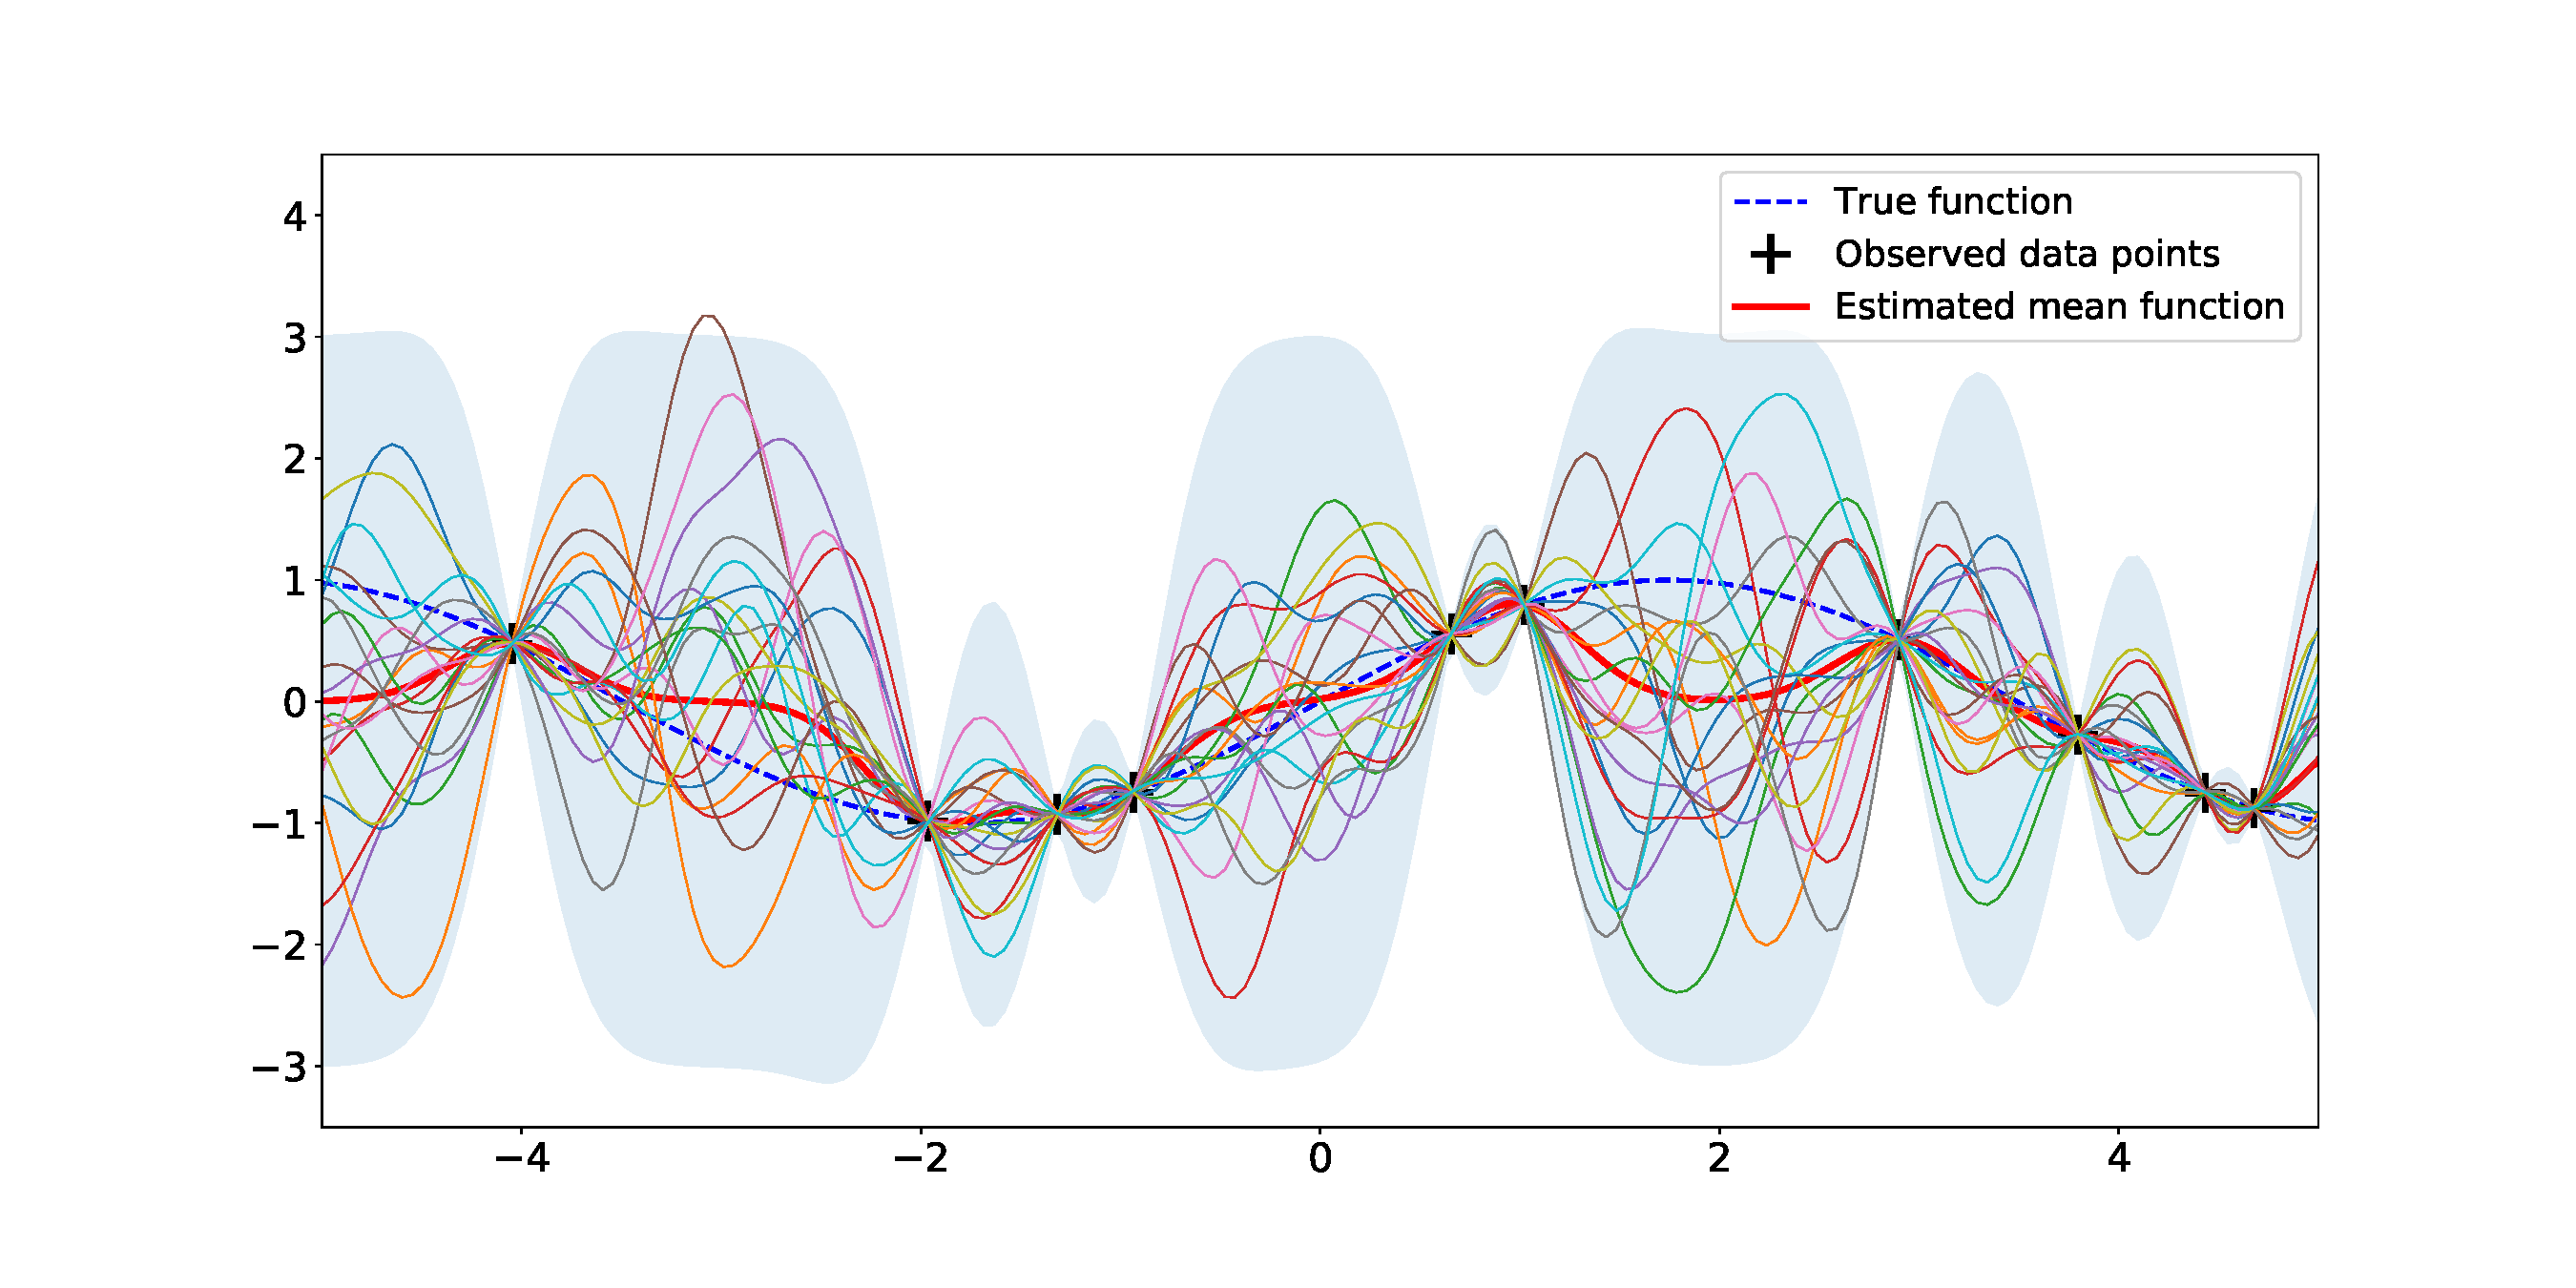
\includegraphics[trim=4.5cm 1.5cm 4.4cm 1.0cm, width=\textwidth]{figs/illustrative_posterior_func.pdf}}}
	\caption{A illustrative example of the standard GPR. The observed data points generated by the blue dotted line (the true function) were plotted as black crosses.  Given the observed/training data points, infinite possible posterior functions were obtained. We plotted 20 samples of these infinite functions with sorted colors. The mean function was obtained by the probability distribution of these functions and plotted as a red solid line. The blue shaded area around the mean function indicates the $3\mu$ prediction variances.}
	\label{FIG:10}
\end{figure}

\subsection{Hyperparameters Optimization}\label{Hyperparameters}

We explained the basics of GPR and implemented a simple example. While in practice, GPR models are more complex than it. Kernel functions play significant roles in GPR. The choice of kernel functions determines almost all the generalization properties of a GP model \cite{duvenaud2016kernel}. There are many covariance functions to choose or make your own for a Gaussian process depending on your specific problem. These criteria include if the model is smooth, if it is sparse, if it can change drastically, and if it needs to be differentiable \cite{duvenaud2014automatic}. More depth information on choosing a kernel/covariance function for a Gaussian process can be found in \cite{duvenaud2014automatic}. In kernels, hyperparameters optimization is essential. Here we will use the most widely used kernel, RBF, as an example to explain the hyperparameters optimization. The general RBF function is given by

\begin{ceqn}
    \begin{align}
        k(\mathbf{x}_i,\mathbf{x}_j) = \sigma_f^2 \exp \Big(-\frac{1}{2l}
         (\mathbf{x}_i - \mathbf{x}_j)^\mathsf{T}
         (\mathbf{x}_i - \mathbf{x}_j) \Big)  \ , \nonumber
    \end{align}
\end{ceqn}
where $\sigma_f$ and $l$ are hyperparameters \cite{duvenaud2014automatic}. The vertical scale $\sigma_f$ describes how much vertically the function can span. The horizontal scale $l$ indicates how quickly the correlation relationship between two points drops as their distance increases. The effect of $l$ was shown in Fig. \ref{FIG:11}. A higher $l$ provided a smoother function and a smaller $l$ gave a wigglier function. 
\\

\begin{figure}[h!]
    \centering
    \subfloat[$l$ = small]{{\includegraphics[trim=3.0cm 1.0cm 3.8cm 2cm, width=0.44\textwidth]{figs/l_small.pdf} }}
    \qquad
    \subfloat[$l$ = medium]{{\includegraphics[trim=2.4cm 1.0cm 3.8cm 2cm, width=0.45\textwidth]{figs/l_medium.pdf} }}
    \qquad 
    \\
    \vspace{0.1cm}
    \subfloat[$l$ = large]{{\includegraphics[trim=3.0cm 1.0cm 3.8cm 2cm, width=0.44\textwidth]{figs/l_large.pdf} }}
    \caption{The function smoothness affected by the horizontal scale $l$ of hyperparameters.}
    \label{FIG:11}
\end{figure}

The optimal hyperparameters $\mathbf{\Theta^*}$ are determined by the log marginal likelihood \cite{Rasmussen2006} as  
\begin{ceqn}
    \begin{align}
        \mathbf{\Theta^*} = \arg\max\limits_{\Theta} \log p(\mathbf{y} \, \vert \, \mathbf{X}, \mathbf{\Theta})  \ . \nonumber
    \end{align}
\end{ceqn}
Thus, considering hyperparameters, a more general equation of predictions at the new testing points is \cite{gpss2019}  
\begin{ceqn}
    \begin{align}
        \mathbf{\bar{f}_*} \, \vert \, \mathbf{X}, \mathbf{y}, \mathbf{X}_*,  \mathbf{\Theta} \sim \mathcal{N} \left(\mathbf{\bar{f}_*}, \text{cov}(\mathbf{f}_*)\right)  \ . \nonumber
    \end{align}
\end{ceqn}
Note that after learning/tuning the hyperparameters, the predictive variance $\text{cov}(\mathbf{f}_*)$ depends on not only the inputs $\mathbf{X}$ and $\mathbf{X}_*$ but also the outputs $\mathbf{y}$ \cite{chen2018priors}. With the optimized hyperparameters $\sigma_f = 0.0067$ and $l = 0.0967$, the regression result of the observed data points in Fig. \ref{FIG:11} was shown in Fig. \ref{FIG:12}. Here, the hyperparameters optimization was conducted by the GPy package, which will be introduced in the next section. 

\begin{figure}[h!]
	\centering
		{{\includegraphics[trim=2.2cm 1.0cm 2.8cm 0.8cm, width=0.74\textwidth]{figs/regression_gpflow.pdf}}}
	\caption{Regression result with the optimized hyperparameters $\sigma_f$ and $l$.}
	\label{FIG:12}
\end{figure}

\subsection{Gaussian processes packages}
This section will review three software packages written in Python for Gaussian processes implementations. One of the most well-known GP packages is GPy \cite{de2017gpflow}. GPy is a maturely developed package with well-documented explanations since 2012. GPy uses NumPy to perform all its computations. For tasks that do not require heavy computations, GPy is sufficient and stable to use. However, GPR is computationally expensive in high dimensional spaces (features more than a few dozens) because it uses the whole samples/features to do predictions. The more observations, the more computations are needed for predictions. A package that includes state-of-the-art algorithms is preferred for efficient implementations of complex GPR tasks. For GPR tasks that are computationally expensive, GPU acceleration is especially useful. GPflow \cite{de2017gpflow} origins from GPy with much of a similar interface. GPflow leverages TensorFlow as its computational backend. GPyTorch \cite{gardner2018gpytorch} is a recently developed package that provides GPU acceleration through PyTorch. It also contains many state-of-the-art Gaussian processes algorithms. Similar to GPflow, GPyTorch provides automatic gradients, thus complex models such as embedding deep neural networks in GP models can be easier developed. 

\section{Summary and Discussion}
A Gaussian process is a probability distribution over possible functions that fit a set of points \cite{Rasmussen2006}. A Gaussian processes regression model provides uncertainty estimations together with prediction values. The prior knowledge of the form of functions can be integrated by using kernel functions.

The GPR model in this tutorial is the standard or vanilla Gaussian processes \cite{frigola2013bayesian}. There are two main constraints with it: 1) The overall computation complexity is $O(N^3)$, where $N$ is the dimension of the covariance matrix $K$. 2) The memory consumption is quadratic. Because of the computation complexity and memory consumption, the standard Gaussian processes model gets stuck quickly. For regression tasks with a big dataset, sparse GP is used to reduce computational complexity \cite{liu2020gaussian}.


%% The Appendices part is started with the command \appendix;
%% appendix sections are then done as normal sections
\appendix
\section{Appendix}
\label{APPENDIX}

The Marginal and Conditional Distributions of MVN theorem: suppose $X=({x}_1,{x}_2)$ is a joint Gaussian with parameters
\begin{ceqn}
    \begin{align}
        {\mu}=\begin{bmatrix}{\mu}_1 \\ {\mu}_2\end{bmatrix} , \ 
        {\Sigma}=\begin{bmatrix} {\Sigma}_{11} & {\Sigma}_{12} \\ {\Sigma}_{21} & {\Sigma}_{22} \end{bmatrix} , \ 
        {\Lambda}={\Sigma}^{-1}=\begin{bmatrix} {\Lambda}_{11} & {\Lambda}_{12} \\ {\Lambda}_{21} & {\Lambda}_{22} \end{bmatrix} \ , \nonumber
    \end{align}
\end{ceqn}
then the marginals are given by
\begin{ceqn}
    \begin{equation}
        \begin{split}
            p({x}_1)= \mathcal{N}({x}_1|{\mu}_1,{\Sigma}_{11}) \ , \\
            p({x}_2)= \mathcal{N}({x}_2|{\mu}_2,{\Sigma}_{22})  \ , \nonumber
        \end{split}
    \end{equation}
\end{ceqn}
and the posterior conditional is given by

\begin{ceqn}
   \begin{equation}\label{eqn:Marginals-and-conditionals-of-an-MVN}
       \begin{split}
        p({x}_1|{x}_2)& =\mathcal{N}({x}_1|{\mu}_{1|2},{\Sigma}_{1|2}) \\
        {\mu}_{1|2}& = {\mu}_1+{\Sigma}_{12}{\Sigma}_{22}^{-1}({x}_2-{\mu}_2) \\
    	               & = {\mu}_1-{\Lambda}_{11}^{-1}{\Lambda}_{12}({x}_2-{\mu}_2) \\
    				   & = {\Sigma}_{1|2}\left({\Lambda}_{11}{\mu}_1-{\Lambda}_{12}({x}_2-{\mu}_2)\right) \\
    	{\Sigma}_{1|2}& = {\Sigma}_{11}-{\Sigma}_{12}{\Sigma}_{22}^{-1}{\Sigma}_{21}={\Lambda}_{11}^{-1} \nonumber
       \end{split}
    \end{equation}
\end{ceqn}
%% \section{}
%% \label{}

%% If you have bibdatabase file and want bibtex to generate the
%% bibitems, please use
%%
\bibliographystyle{elsarticle-num} 
\bibliography{bibliography}

%% else use the following coding to input the bibitems directly in the
%% TeX file.

% \begin{thebibliography}{00}

% %% \bibitem{label}
% %% Text of bibliographic item

% \bibitem{}

% \end{thebibliography}


\end{document}
\endinput
%%
%% End of file `elsarticle-template-num.tex'.
